\documentclass[a4paper, 12pt]{article}
% \documentclass[a4paper, 12pt]{beamer}
% \documentclass[a4paper, 12pt]{report}
% \documentclass[a4paper, 12pt]{book}
% \documentclass[a4paper, 12pt]{letter}
% memoir, komma-script

\newcommand{\EPA}{{\LARGE C. B. D.}}
\newcommand{\zvyrazni}[1]{\textbf{\textit{#1}}}

\usepackage[czech]{babel}
\usepackage[T1]{fontenc}
\usepackage[a4paper, margin=2cm]{geometry}
\usepackage{graphicx}
\usepackage[unicode]{hyperref} % unicode propisuje diakritiku do menu

\title{Hrabáč kapský}
\author{Petr Kotlan\thanks{Univerzita J. E. Purkyně}}
\date{14. 3. 2023}

\begin{document}

\maketitle

\tableofcontents

\verb#\LaTeX# vysází slovo \LaTeX


\section{Úvod}
Hrabáč kapský (\emph{Orycteropus afer}) je středně velký savec původem z Afriky. Ve starší české literatuře,
například v cestopisech Emila Holuba nebo starších vydáních Brehmova \textit{Života zvířat} je nazýván kuťoš (od slovesa kutat)
nebo \textbf{takaru}, což je domorodý název pocházející z oblasti Etiopie.
Anglické jméno Aardvark \texttt{[a:dva:k]} pochází z afrikánštiny a znamená \uv{(pod)zemní sele},
jelikož původní osadníci z Evropy ho považovali za zvíře podobné praseti
(ačkoliv hrabáči nejsou blízcí příbuzní prasat).
Ve východní Africe je znám pod svahilským jménem \textsc{Kukukifiku}.

\begin{verbatim}
    for i in range(100):
    print(i)
\end{verbatim}


\EPA

\zvyrazni{test}

\textsf{Hrabáč kapský} je poslední přežívající druh z řádu hrabáčů (Tubulidentata) a jeho jediné >>čeledi<< hrabáčovitých.
Hrabáč byl původně řazen do řádu chudozubých, a to pro svou vnější podobnost s mravenečníkem.
Výzkum však prokázal, že si tato zvířata příbuzná nejsou a podobnosti v jejich stavbě
těla jsou výsledkem konvergentní evoluce v důsledku adaptace na stejný typ potravy -- termity.
Z podobných důvodů má hrabáč společné rysy s vačnatými bandikuty. Nejbližší příbuzní hrabáče
jsou vyhynulé rody Leptorycteropus a Myorycteropus, nejbližší žijící příbuzní afrosoricidi nebo bércouni.

Ve střevě hrabáče kapského parazituje vrtejš Oligacanthorhynchus longissimus,
který je s délkou až 93~cm největším druhem vrtejše.

\section{Popis a morfologie}

Hrabáč kapský je zavalitě stavěný savec, dosahující hmotnosti až 60 kg, délky těla 110--130 cm a délky ocasu 70 cm.
Mohutné tělo hrabáče je téměř lysé, pouze na hřbetě ho pokrývají řídké štětiny.
Zbarvení je béžové, na břiše a hlavě až narůžovělé.
Končetiny s mohutnými drápy jsou sloupovité, zadní delší než přední, silný, málo pohyblivý ocas, podobný klokanímu, zvířeti umožňuje, aby se postavilo na zadní nohy.
Hlava hrabáče je protáhlá a její přední část se podobá prasečímu rypáku. Oči jsou malé, naproti tomu boltce dlouhé a blanité, tvarově podobné zaječím. Ve spánku je zvíře skládá podél hlavy.
Nejtypičtějším znakem hrabáče je zcela ojedinělá stavba chrupu, během vývoje došlo k regresivnímu vývoji chrupu jako i některých zástupců chudozubých a luskounů (proto chybné zařazení).
Chrup hypselodontního typu, zuby stále dorůstají a jsou bezkořenné.
Varlata mají samci uložena v břišní dutině, podobně jako sloni, nemají šourek.
Na předních končetinách došlo k redukci prstů na 4, zadní končetiny jsou pětiprsté.

\begin{figure}
    \centering
    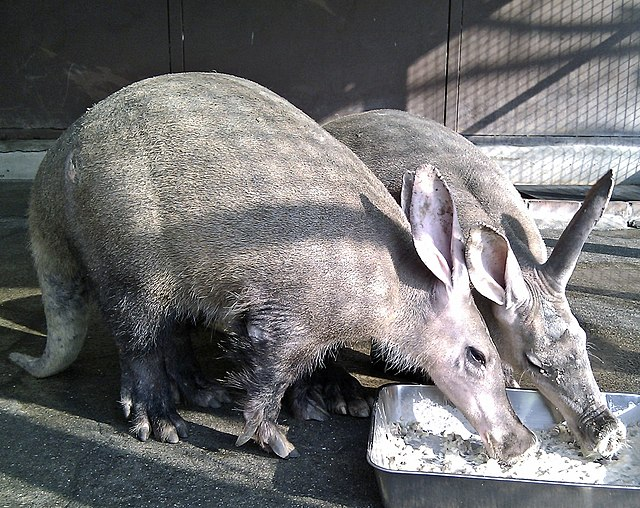
\includegraphics[width = \textwidth]{obrazky/hrabac_kapsky.jpg}
    \caption{Hrabáč kapský}
\end{figure}


\section{Rozšíření}

Hrabáč kapský se vyskytuje v Africe na jih od Sahary, především v savanách a buši, kde se vyskytuje dostatek termitů.
V Botswaně se vyskytuje i v polopoušti Kalahari, naproti tomu v Etiopii vystupuje poměrně vysoko do hor.
Vyhýbá se deštným pralesům.

\section{Způsob Života}

Hrabáč kapský je aktivní především v noci, den přespává ve své noře. Je samotář.
Ze smyslů hrabáče je nejlepší čich a sluch, zrak je poměrně slabý. Dlouhé boltce v klidu drží vzpřímeně,
ale dovede je složit a uzavřít tak zvukovody. Zvláštně stavěným čenichem vyhledává kořist.
Kolem nozder má husté chlupy, které je chrání při hrabání. Hrabáč je výborně přizpůsoben k hloubení nor.
Nory hloubí pomocí svých silných předních nohou, které jsou opatřeny drápy, vyhrabanou zeminu odtlačuje zadníma nohama.
Pomocí silných drápů také rozhrabává termitiště a mraveniště, jejichž obyvateli se živí.

\section{Potrava}

Hrabáč kapský se v přírodě živí především mravenci a termity, jejichž hnízda rozhrabává
silnými drápy a vyplašený hmyz pak nalepuje dlouhým jazykem. V zajetí je složení krmení individuální,
skládá se z mnoha komponentů, s vysokým obsahem bílkovin.
(mleté vařené hovězí maso, žloutky, mléko, banány...)

\section{Rozmnožování}

Samice rodí jen jediné mládě o hmotnosti přibližně 1,6 kg. Březost trvá 243 dní.
Mládě saje 4 měsíce. V zajetí se dožívá průměrně 21--23 let.

\section{Chov v zoo}

Patří mezi vzácně chované druhy. První jedinec byl dovezen do londýnské zoo v roce 1869.
První rozmnožení bylo zaznamenáno v roce 1962 v zoo Frankfurt nad Mohanem.
První úspěšný odchov (umělý) se podařil v roce 1967 v Miami Crandon Park ve Spojených státech amerických.
První přirozený odchov následoval roku 1969 v zoo Artis Amsterdam.
V říjnu 2019 chovalo hrabáče kapského přibližně 25 evropských zoo,
přičemž odchovy jsou zaznamenávány asi v šesti institucích. V Česku je lze spatřit v:

\begin{itemize}

    \item Zoo Praha (od 1979, několikrát se zde rozmnožil, naposledy 10. 7. 2022)
          \begin{itemize}
              \item První položka
              \item Druhá položka
              \item Třetí položka
          \end{itemize}
    \item ZOO Dvůr Králové (od 2014, 2017 se zde narodilo historicky první mládě)
    \item Zoo Olomouc (od roku 2017 samec, od března 2018 samice – odchov ze Zoo Praha)
    \item Zoo Plzeň (od roku 2019 samice ze Zoo Antverpy)

\end{itemize}

\begin{enumerate}

    \item Zoo Praha (od 1979, několikrát se zde rozmnožil, naposledy 10. 7. 2022)
          \begin{enumerate}
              \item První položka
              \item Druhá položka
              \item Třetí položka
          \end{enumerate}
    \item ZOO Dvůr Králové (od 2014, 2017 se zde narodilo historicky první mládě)
    \item Zoo Olomouc (od roku 2017 samec, od března 2018 samice – odchov ze Zoo Praha)
    \item Zoo Plzeň (od roku 2019 samice ze Zoo Antverpy)

\end{enumerate}

\begin{description}
    \item[zoo Praha] (od 1979, několikrát se zde rozmnožil, naposledy 10. 7. 2022)
\end{description}

\subsection[Praha]{Chov v Zoo Praha}

Chov hrabáče kapského v pražské zoo započal v roce 1979. Jednalo se o první zvířata tohoto druhu v Československu. Tehdy přišly ze Spojeného království dvě samice (Bojsa a Nebojsa). Po úhynu druhé ze samic došlo k dovozu samce – geneticky cenného z volné přírody, konkrétně z Namibie.[7] První odchované mládě přišlo na svět o dva roky později – v roce 1989[8]. Další odchovaná mláďata následovala v roce 1994 a 2004.[8]

Současný chovný samec Draco je vnukem původního samce Táty.
Samice Kvída přišla do Prahy v roce 2006 a pochází z nizozemské zoo v Arnhemu, kde se 1. 2. 2005 narodila.
První dvě společná mláďata Draca a Kvídy se nepodařilo odchovat, další pokusy však již byly úspěšné. 26. 7. 2015 se narodil samec a následně dostal jméno Kito.
Mládě pokřtili Taťána Kuchařová a Ondřej Brzobohatý. Dnes Kito žije v Dánsku (zoo Randers). 20. 8. 2016 přišla na svět samička Nyota, v překladu hvězda.
Jméno vybrali čtenáři Blesk.cz. Samička opustila zoo Praha na počátku března 2018 a zamířila do Olomouce. Zatím poslední mládě (samička) se narodilo 22. 4. 2018.
10. 6. 2018 byla pokřtěna hereckým párem Igor Bareš a Antonie Talacková a dostala jméno Sawa. V březnu 2019 odešla do britského Shepreth Wildlife Parku. Do počátku roku 2019 se tak podařilo odchovat šest mláďat.

Hrabáči jsou v zoo Praha od roku 2001 chováni v pavilonu Africký dům v severní části zahrady. Dříve byli v areálu karantény a k vidění byli jen za letních dnů.

\section{Hrabáči v kultuře}

\subsection{knihy}

Thomas Cathcart, Daniel Klein: Aristotle and an Aardvark Go to Washington: Understanding Political Doublespeak through Philosophy and Jokes (bestseller, USA, 2008)
Masopustová a kolektiv. Chov exotických zvířat (2009). Česká zemědělská univerzita. ISBN 978-80-213-1916-5
TV seriál
TV seriál BBC: Červený trpaslík, Série IV, Epizoda 1: „Kamila“

\end{document}